% Springer LNCS version (llncs). Build: tectonic springer.tex
% Shared content: abstract.tex, body.tex, appendix.tex, macros.tex, references.bib
\documentclass[runningheads]{llncs}
\usepackage[T1]{fontenc}
% Shared packages and macros (class-independent). Included by all wrappers.
\usepackage{amsmath,amssymb}
\usepackage{booktabs}
\usepackage{tabularx}
\usepackage{multirow}
\usepackage{xcolor}
\usepackage{graphicx}
\usepackage{tikz}
\usetikzlibrary{arrows.meta,positioning}
\usepackage{pgfplots}
\pgfplotsset{compat=1.17}
\usepgfplotslibrary{groupplots}
\setlength{\emergencystretch}{1em}
\newcolumntype{Y}{>{\raggedright\arraybackslash}X}
\newcommand{\choice}{\texttt{choice}}
\newcommand{\noul}{\texttt{noul}}
\newcommand{\score}{\texttt{score}}
\newcommand{\astar}{a^{*}}
\newcommand{\papertitle}{Jev's Structured Outputs Do Not Imply Compatible Uncertainty:
An Empirical Study of Confidence Signals in a Multi-Step Decision Workflow}

\usepackage{float}
\setlength{\emergencystretch}{3em}
\usepackage[hidelinks]{hyperref}
\usepackage[capitalise]{cleveref}
\newcommand{\citep}[1]{\cite{#1}}
\newcommand{\para}[1]{\paragraph{#1.}}
\newenvironment{colfigure}{\begin{figure}[t]}{\end{figure}}
\newenvironment{coltable}{\begin{table}[t]}{\end{table}}
% Appendix tables print exactly where written (no floating into the references).
\newenvironment{apptable}{\begin{table}[H]}{\end{table}}
\newenvironment{widefigure}{\begin{figure}[t]}{\end{figure}}
\newenvironment{widetable}{\begin{table}[t]}{\end{table}}

\title{Jev in a Multi-Step Workflow}
\subtitle{Predicting Failures Is Not Knowing Which Reviews Pay}
\titlerunning{Jev in a Multi-Step Workflow}
% For double-blind review, replace the author and institute blocks.
\author{Thejas P Rao\inst{1} \and Tushar M\inst{2}}
\authorrunning{T. P. Rao and T. M}
\institute{\email{thejasrao262003@gmail.com} \and \email{tusharm3040@gmail.com}}

\begin{document}
\maketitle
\begin{abstract}
% Shared abstract (included by main.tex, ieee.tex, springer.tex)
Structured-output decision APIs return well-typed answers together with
numeric confidence, and it is tempting to treat those numbers as
interchangeable probabilities that can be composed across the steps of a
workflow. We examine that practice for Jev, TypeSafe's structured
decision model, and its three decision primitives: a categorical
\choice{}, a binary \noul{} and an ordinal \score{}. TypeSafe documents
Jev's confidence as a summary of the output distribution rather than a
calibrated estimate of accuracy. We measure what that distinction means
once the primitives are composed. The primitives are chained into a three-step triage
workflow (route, assess, rate severity). We evaluate on controlled
constructed items, on 202 Mozilla bugs labeled by triage and on 240 Linux
kernel bugs labeled by their reporters, using 4{,}584 API calls in the main
real-data runs. Three findings hold on both trackers.
First, the primitives' confidence signals have distinct failure modes.
\choice{} confidence is saturated (85--96\% of real bugs at $\geq 0.90$)
yet discriminative (AUROC 0.90 [0.83, 0.96] and 0.98 [0.95, 1.00]).
\noul{}'s confidence-like value is uninformative (AUROC 0.53
[0.42, 0.65] and 0.41 [0.32, 0.50]). \score{}'s confidence is flat across
true severity levels.
Second, fixed confidence thresholds designed on constructed data lose
their intended selectivity on real text: a cut that escalated 73\% of
constructed items (target 67\%) escalated 88\% and 78\% of real bugs
(targets 41--42\%).
Third, \score{} compresses severity toward the middle level, consistent
with central-tendency bias reported for LLM raters in other domains, and
its confidence gives no indication of it.
In exploratory analyses, the composition rules we tested did not
consistently identify which cases to escalate: ranking escalations by
composed confidence did no better than random selection on either
tracker (one borderline worse-than-random estimate did not replicate), and
the intervals cannot exclude a modest signal. We
also show that a natural comparison of confidence-based against
decision-based composition is confounded when the target action is
itself a function of the decisions. The corrected comparison is
pre-registered for a controlled follow-up that has not yet been run.

\keywords{Uncertainty quantification \and Calibration \and Structured outputs
\and Decision workflows \and Escalation \and Bug triage}
\end{abstract}
% Shared body (included by main.tex, ieee.tex, springer.tex)
%======================================================================
\section{Introduction}
%======================================================================

A model can return a perfectly valid, well-typed structured response and
still make the wrong decision. When several such decisions are chained
into a workflow, errors at one step propagate to the next. A common hope
is that each step's reported confidence can be composed into a
workflow-level signal that says when to hand a case to a human.

Prior work has benchmarked Jev's primitives and calibration on single
tasks \citep{deusser2026jev,meng2026jevaudit,denney2026jev}, and recent
work has examined uncertainty across multi-step agent trajectories
\citep{lin2026uqagents}. We study a different, operational question.
\emph{When a workflow chains heterogeneous typed decisions, which signals
identify the cases where it fails, and can those signals identify the
specific costly errors for which human review is worthwhile?} The two
halves can come apart: a signal can rank failures well and still not say
which reviews pay. Heterogeneity matters because Jev exposes three primitives whose uncertainty is
\emph{structurally} different. \choice{} returns a
distribution over labels plus a scalar confidence. \score{} returns an
ordinal distribution plus a scalar confidence. \noul{} returns a single
probability with no separate confidence field. Treating these numbers as
one kind of quantity is a modeling assumption, and this paper tests it.

\para{What TypeSafe documents} TypeSafe's documentation describes
Jev's \texttt{confidence} for \choice{} and \score{} as a number that
``collapses'' the output distribution into a value between 0 and 1. It
is 1 when all probability is on one outcome and 0 when probability is
spread evenly. The documentation calls this ``one reasonable way to
summarize a distribution, not the only one'', and advises setting
thresholds from one's own data \citep{typesafe2026confidence}. For
\noul{}, it returns ``a single probability'' with ``no separate
\texttt{confidence}''. Our results are therefore not a test of a
calibration claim. They are a measurement of how these documented
concentration statistics behave as escalation signals when Jev's
primitives are chained, which the documentation leaves open.

\para{Contributions} The main findings concern workflow-level prediction
and its decision utility.
\begin{enumerate}
  \item \textbf{Workflow failure prediction} (\cref{sec:heldout,sec:crossmodel},
  pre-registered). A frozen decision-feature estimator ranks wrong workflow
  actions better than final-step confidence on 500 new bugs. The gap
  replicates across five evaluated models from four sources, and Jev's
  frozen estimator transfers unchanged to an independently trained
  Jev-style model. Most of the signal is the chosen action's historical
  error rate.
  \item \textbf{Prediction is not intervention utility} (\cref{sec:intervention},
  pre-registered). At a 10\% review budget and the pre-registered costs,
  that predictive signal does not yield a lower cost than
  confidence-ranked review, and no strategy beat no review; an
  exploratory sensitivity analysis shows that whether review pays depends
  on the cost ratio. An oracle shows the reason: the expensive errors exist,
  but the signals we tested could not isolate them within an action. A
  case-level score developed on training bugs did not meet a
  pre-registered feasibility criterion under the natural bug mix, so the
  planned confirmatory study was stopped before any new data.
  \item \textbf{Supporting evidence on the primitives}
  (\cref{sec:char,sec:transfer,sec:real,sec:comp}). Inside this workflow,
  the three primitives' confidence signals behave differently; fixed
  thresholds set on constructed content lose their selectivity on real
  text; \score{} compresses severity on two trackers with different
  labeling processes; and confidence-based escalation rules did not
  consistently beat random selection (exploratory, with a confound we
  identify). Primitive-level calibration of Jev has been studied
  elsewhere on single tasks
  \citep{deusser2026jev,meng2026jevaudit}; these results are the
  foundation for the workflow study rather than its main claim.
  \item \textbf{Method} (\cref{sec:method}). A pre-registration and audit
  process that caught six design or implementation defects, most of them
  before any evaluation data existed.
\end{enumerate}

\para{Non-claims} We make no claim about general calibration, other
Jev versions or other APIs, domains beyond software bug triage, or real-world
operational benefit.

%======================================================================
\section{Related work}
%======================================================================

\para{Evaluations of Jev and open decision models} Jev has been
benchmarked zero-shot on 37 datasets (346{,}009 requests), where its
\choice{} probabilities were well calibrated and supported selective
prediction, while its binary probabilities ranked well but sat poorly
relative to a 0.5 threshold, and thresholds tuned on training data
improved F1 \citep{deusser2026jev}. A calibration audit with released per-item
outputs (described by its author as exploratory) compared Jev with open
and general-purpose classifiers on SST-2 and AG News
\citep{meng2026jevaudit}. It found that calibration changed with the
question form (a yes/no form was underconfident, a choice form close to
calibrated), that 71.6\% of four-class answers sat at exactly 1.00, so
a threshold on the top-class probability had only 53 operating points,
that one fitted temperature removed most miscalibration, and that no
threshold on Jev's scores certified a 5\% automatic tier on the
four-class task under its procedure; and a comparison on seven
political-science replications found its calibration advantage over
other models not consistent \citep{denney2026jev}. An early evidence
audit of 28 papers on typed decision models found no independent
accuracy advantage yet for the typed readout over comparable
label-probability readouts, and proposed an evaluation checklist
\citep{tang2026typed}. Open instruction-tuned models can produce
Jev-like decisions by reading answer-label logits in one forward pass
\citep{geuter2026innerjev}, the same kind of readout we use for the
general models in \cref{sec:crossmodel}. These studies evaluate single
requests; none studies \score{} inside a workflow, composition of
dependent decisions, or the cost of human review. Our results agree with
them where they overlap: \choice{} confidence is saturated yet
discriminative, and thresholds must be validated on the target data,
which our transfer result shows directly. On \noul{} the measures
differ. The audits report calibration and accuracy on sentiment, where
the yes/no form was accurate and recalibratable; on our regression
question, \noul{}'s probability did not discriminate its own correctness
(AUROC near or below 0.5). Binary-probability quality therefore looks
task-dependent.

\para{Calibration of single decisions} Post-hoc calibration
\citep{platt1999probabilistic,naeini2015bbq} and the miscalibration of
modern networks \citep{guo2017calibration} are well studied, and
confidence estimation for language models has been surveyed in
\citep{geng2024survey}.

\para{Selective prediction and deferral} Risk--coverage trade-offs
and reject options \citep{elyaniv2010selective,geifman2017selective,geifman2019selectivenet},
learning to defer \citep{madras2018predict} and prediction sets in
human--AI teams \citep{babbar2022predsets} address \emph{one} decision.
Closest to our intervention result, recent work argues that error risk is
not review value under bounded review budgets: review priority should
depend on wrongness, repairability, impact and cost, and ranking by
review value left less residual error than ranking by risk on a
question-answering benchmark \citep{park2026riskreview}. Our
intervention finding is an instance of that distinction in a dependent
typed-decision workflow, with a frozen cost table and pre-registered
tests.

\para{Conformal methods and composition} Conformal prediction
\citep{angelopoulos2021gentle} and conformal risk control
\citep{angelopoulos2024crc} give distribution-free guarantees. Composition
across stages has been studied for two stages \citep{zhang2025modular}
and for multi-stage NLP and LLM pipelines, where errors compound across
stages and independently calibrated stages lack a joint coverage
guarantee \citep{kotte2026pasc}.
Error propagation through pipeline steps has also been quantified
\citep{chowdhury2019error}. Classical reliability theory composes
component reliabilities \citep{barlow1965reliability}.

\para{Cascades and escalation} Cascades route a \emph{single} query
through model tiers. Prior work studies early abstention
\citep{zellinger2025early}, the optimal depth and deferral thresholds of
cascades \citep{bouchard2026escalation}, conformal cascades
\citep{dou2026conformalcascade}, confidence tuning \citep{rabanser2025gatekeeper}
and judges with escalation guarantees \citep{jung2025trust}.

\para{Combining confidence across components} Fixed combination
rules such as the product rule are classical
\citep{kittler1998combining}. The product rule's usual justification
assumes conditional independence and comparable probability scales, and
these are precisely the assumptions our strategy S2 makes implicitly. At
the system level, a recent taxonomy argues that uncertainty in LLM
applications must be studied across the whole compound system, as it
propagates within models, across system components and through
socio-technical processes \citep{xia2026propagation}. Cost-sensitive
deferral to multiple experts under workload limits \citep{alves2024defer}
is closely related to the budgeted escalation setting our follow-up uses.

\para{Ordinal outputs and central tendency} LLM raters have been
reported to compress ordinal scores toward the middle of the scale, for
example in clinical scoring, where prompt changes did not remove the
effect \citep{zhang2026centraltendency}. Few-label calibration of ordinal
LLM outputs models such flattening explicitly \citep{wang2026cordial}.
Our severity result is consistent with this literature. What we add is
that it appears in bug triage, against two labeling processes, and that
the primitive's own confidence gives no sign of it.

\para{Agents and trajectories} Closest to our workflow framing, a counterexample
shows that step-level calibration need not imply trajectory-level
calibration for LLM agents, and step errors are empirically coupled along
trajectories \citep{lin2026uqagents}. Related work calibrates agent
trajectories \citep{zhang2026agentic} and studies uncertainty propagation
in multi-step agentic decisions \citep{duan2025uprop}.

\para{Positioning} Prior work benchmarks Jev's primitives on single
requests, studies calibration of single decisions, cascades of the
\emph{same} decision and agent trajectories, and argues in general that
risk differs from review value. Our contribution is narrower and
empirical: in a dependent workflow of three \emph{structurally
different} typed decisions, against real labels, held-out data and five
evaluated models, we test which signals predict workflow failure and
whether they identify the costly errors that make human review
worthwhile. We are not aware of prior work with this specific design, but
we make no priority claim. Our literature search was web-based, did not
systematically cover reliability engineering or HCI escalation research,
and the Jev literature is growing quickly: the studies cited above
appeared in September and October 2026.

%======================================================================
\section{Setting}
\label{sec:setting}
%======================================================================

\para{Jev and repeats} All calls go to the TypeSafe API with model
\texttt{jev-latest}, which resolved to \texttt{jev-1.13.0} in every one of
our calls. Each node is called three times, and the three
answers are reduced to one decision. For \choice{} and \score{} we take
the modal decision with a tie tolerance of 0.02; a node with no
two-of-three majority is \emph{repeat-unstable}. For \noul{} we threshold
the mean probability at 0.5, and its confidence-like value is
$2\,|\bar{p}-0.5|$.

\para{Workflow} Node~1 (\choice{}) routes the incident to a
network or storage subsystem. Node~2 (\noul{}) assesses a binary
property: customer impact on constructed data, regression on real bugs.
Node~3 (\score{}) rates severity on three levels. Each node reads the
evidence plus the upstream decisions, appended by a fixed adapter
(\cref{fig:workflow}).

\begin{widefigure}
\centering
\resizebox{\linewidth}{!}{%
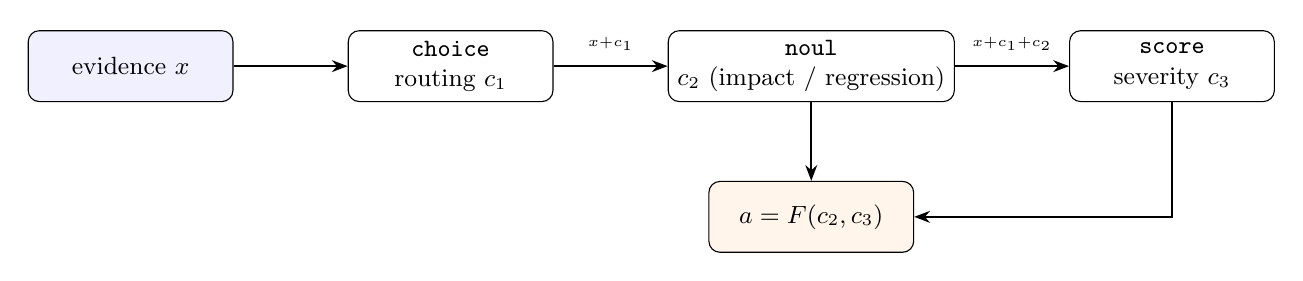
\begin{tikzpicture}[node distance=1.45cm, every node/.style={font=\small},
  box/.style={draw, rounded corners, minimum width=2.6cm, minimum height=0.9cm, align=center},
  arr/.style={-{Stealth[length=2mm]}, thick}]
\node[box, fill=blue!6] (ev) {evidence $x$};
\node[box, right=of ev] (c) {\choice{}\\ routing $c_1$};
\node[box, right=of c] (n) {\noul{}\\ $c_2$ (impact / regression)};
\node[box, right=of n] (s) {\score{}\\ severity $c_3$};
\node[box, below=1.0cm of n, fill=orange!8] (f) {$a = F(c_2, c_3)$};
\draw[arr] (ev) -- (c);
\draw[arr] (c) -- node[above=2pt]{\tiny $x{+}c_1$} (n);
\draw[arr] (n) -- node[above=2pt]{\tiny $x{+}c_1{+}c_2$} (s);
\draw[arr] (n) -- (f);
\draw[arr] (s) |- (f);
\end{tikzpicture}}
\caption{The three-step workflow. Each node is called three times. The
action rule $F$ uses only $c_2$ and $c_3$.}
\label{fig:workflow}
\end{widefigure}

\para{Target action} The target is $\astar = F(c_2^{*}, c_3^{*})$,
where $F$ maps an \emph{unclear} $c_2$ to \emph{request more evidence},
$c_3 = 2$ to \emph{escalate}, $c_3 = 1$ with $c_2 = 1$ to \emph{defer},
and everything else to \emph{accept} (\cref{tab:F}). $F$ is a construct
we defined, not an independently validated outcome, and every strategy
result is conditional on it.

\para{Strategies}
\begin{itemize}
  \item \textbf{S1:} $F$ applied to the node decisions.
  \item \textbf{S4a:} S1 plus escalation on repeat instability.
  \item \textbf{S2:} escalate the $\lceil qn\rceil$ instances with the
  lowest product of per-node confidences and accept the rest. Here $q$
  is the share of non-accept targets.
  \item \textbf{S5:} the same, ranked by per-primitive rank-normalized
  uncertainty.
  \item \textbf{2h / 5h:} S1 plus confidence-ranked escalation of a fixed
  10\% budget.
  \item \textbf{R:} the same budget escalated at random.
\end{itemize}
\para{Statistics} Agreement rates carry Wilson 95\% intervals.
AUROCs use the Mann--Whitney estimator, with 95\% percentile bootstrap
intervals over bugs ($B = 2{,}000$, fixed seed). Bugs are distinct
reports with no shared unit, so we resample bugs. Paired strategy
comparisons use the exact McNemar test on discordant pairs, and the
difference in $P(Y_{\text{decision}})$ gets a bootstrap interval. Within
every resample, the set-relative rankings (S2, 2h) are recomputed. We
compare the two trackers through the difference of their paired
differences, with independent bootstraps per tracker. We do not compare
their $p$-values. For budgeted overrides, the reference is the
\emph{exact} expected cost of $k$ random overrides. The randomization
$p$-value (10{,}000 random $k$-subsets) is conditional on the evaluated
bugs, and a bootstrap interval over bugs gives the sampling uncertainty.
An interval that covers the null value is read as \emph{no evidence of an
effect}, not as evidence of no effect. The scripts are
\texttt{paper\_statistics.py} and \texttt{mozilla\_exploratory\_analysis.py}.

\para{Outcomes} Outcomes are $P(Y_{\text{decision}})$, the probability that the action
equals $\astar$, and the cost under a frozen matrix (\cref{tab:cost}),
in which a wrong \emph{accept} costs 6--10, any other mismatch 1, and each
escalation an extra 1 for human time.

%======================================================================
\section{Characterization: incompatible uncertainty semantics}
\label{sec:char}
%======================================================================

\begin{widetable}
\centering
\caption{Per-primitive behavior of the confidence signal. AUROC is for
predicting the node's own agreement with the reference label, with 95\% bootstrap intervals.}
\label{tab:char}

\small
\begin{tabularx}{\linewidth}{l Y Y Y}
\toprule
 & Constructed items & Mozilla ($n{=}202$, triage) & Kernel ($n{=}240$, reporter) \\
\midrule
\choice{} & High-confidence error subgroup: mean confidence 0.915, accuracy 0.333 ($n{=}6$)
 & 85\% at $\geq0.90$, agreeing 0.96; AUROC 0.90 [0.83, 0.96]; ECE 0.05
 & 96\% at $\geq0.90$, agreeing 0.99; AUROC 0.98 [0.95, 1.00]; ECE 0.02 \\
\addlinespace
\noul{} & 24/24 correct, confidence below accuracy in every bin
 & Agreement flat across bands (0.71--0.84); AUROC 0.53 [0.42, 0.65]; ECE 0.36
 & Non-monotonic (0.58--0.93); AUROC 0.41 [0.32, 0.50]; ECE 0.36 \\
\addlinespace
\score{} & Tracks the most severe sentence (6/6); confidence varies by 0.173 with sentence order alone (1 of 3 items)
 & Confidence $\approx$0.6 at every true level; AUROC 0.58 [0.50, 0.66]
 & Confidence 0.65 / 0.62 / 0.61 by true level; AUROC 0.57 [0.50, 0.64] \\
\bottomrule
\end{tabularx}

\end{widetable}

\Cref{tab:char} and \cref{fig:reliability} show three incompatible profiles. \choice{}'s confidence
is almost always near 1.0. It still discriminates, because the rare
low-confidence answers are where its errors are. The high-confidence
error subgroup found on deliberately ambiguous constructed items does not
recur on real text (2 of 6 kernel errors are at $\geq 0.90$). \noul{}'s
confidence-like value carries no usable information about correctness on
either tracker. Its Mozilla interval covers 0.5, and its kernel interval
lies at or just below 0.5 (weakly anti-informative). \score{}'s confidence does not vary with the true level,
so it gives no warning of the systematic bias in \cref{sec:real}. Any
composition rule that multiplies or averages these numbers inherits this
mix.

\begin{widefigure}
\centering
\begin{tikzpicture}
\begin{groupplot}[group style={group size=4 by 1, horizontal sep=0.75cm},
  width=0.27\linewidth, height=4.0cm, xmin=0, xmax=1, ymin=0, ymax=1.05,
  xtick={0,0.5,1}, ytick={0,0.5,1}, grid=major, grid style={gray!20},
  xlabel={\scriptsize confidence}, title style={font=\small},
  tick label style={font=\scriptsize}, label style={font=\scriptsize}]
\nextgroupplot[title={Mozilla \choice{}}, ylabel={\scriptsize agreement}]
\addplot[gray, dashed, domain=0:1] {x};
\addplot[blue, thick, mark=*, nodes near coords, point meta=explicit symbolic,
  nodes near coords style={font=\tiny, anchor=north west}] table[x=conf, y=acc, meta=n] {fig_rel_mozilla_choice.dat};
\nextgroupplot[title={Mozilla \noul{}}]
\addplot[gray, dashed, domain=0:1] {x};
\addplot[orange, thick, mark=square*, nodes near coords, point meta=explicit symbolic,
  nodes near coords style={font=\tiny, anchor=south}] table[x=conf, y=acc, meta=n] {fig_rel_mozilla_noul.dat};
\nextgroupplot[title={Kernel \choice{}}]
\addplot[gray, dashed, domain=0:1] {x};
\addplot[blue, thick, mark=*, nodes near coords, point meta=explicit symbolic,
  nodes near coords style={font=\tiny, anchor=north west}] table[x=conf, y=acc, meta=n] {fig_rel_kernel_choice.dat};
\nextgroupplot[title={Kernel \noul{}}]
\addplot[gray, dashed, domain=0:1] {x};
\addplot[orange, thick, mark=square*, nodes near coords, point meta=explicit symbolic,
  nodes near coords style={font=\tiny, anchor=south}] table[x=conf, y=acc, meta=n] {fig_rel_kernel_noul.dat};
\end{groupplot}
\end{tikzpicture}
\caption{Reliability diagrams (five equal-width confidence bins, bins with
$n \geq 5$; the label is $n$; dashed line: perfect calibration). \choice{}
puts nearly all bugs in its top bin, and that bin is accurate. \noul{}'s
confidence-like value $2|\bar p - 0.5|$ sits far \emph{below} its agreement
(underconfidence), and agreement does not rise with it.}
\label{fig:reliability}
\end{widefigure}


%======================================================================
\section{Fixed thresholds lose their selectivity on real text}
\label{sec:transfer}
%======================================================================

\begin{colfigure}
\centering
\begin{tikzpicture}
\begin{axis}[ybar, bar width=7pt, width=0.9\linewidth, height=4.6cm,
  symbolic x coords={Pilot,Mozilla,Kernel}, xtick=data, ymin=0, ymax=110,
  ylabel={\% of instances}, enlarge x limits=0.25, ytick={0,25,50,75,100},
  grid=major, grid style={gray!20}, tick label style={font=\scriptsize},
  label style={font=\scriptsize},
  legend style={font=\scriptsize, at={(0.5,1.02)}, anchor=south, legend columns=3, draw=none},
  nodes near coords, nodes near coords style={font=\tiny, rotate=90, anchor=west},
  point meta=y, every node near coord/.append style={/pgf/number format/.cd, fixed, precision=0}]
\addplot[fill=blue!55] table[x=set, y=trigger] {fig_transfer.dat};
\addplot[fill=orange!70] table[x=set, y=cut] {fig_transfer.dat};
\addplot[fill=gray!45] table[x=set, y=target] {fig_transfer.dat};
\legend{\choice{} $\geq$0.90 fires, 0.5 cut escalates, target share}
\end{axis}
\end{tikzpicture}
\caption{Selectivity of the two fixed-threshold rules, set on constructed
data and measured on each rule's own input signals. The trigger fires on
85--96\% of instances everywhere. The product cut is near its target on
the constructed pilot and far above it on real text.}
\label{fig:transfer}
\end{colfigure}

The rules in \cref{fig:transfer} fail in two different ways. On real
text the trigger fired on 85\% (Mozilla) and 96\% (kernel) of bugs, and
the product cut escalated 88\% and 78\% against targets of 41\% and 42\%
(constructed pilot: 27/30 fired; 73\% escalated against 67\%). The \choice{}
trigger is non-selective \emph{everywhere}, because \choice{} confidence
is saturated: that is a design failure, visible only once measured. The
product cut is \emph{distribution-sensitive}. It was near its target on
constructed data and far from it on real data, because real text pulls
\noul{} toward 0.5 and so pulls the product down. A fixed threshold
carries the confidence scale of the data it was set on, and our
constructed data was too clean to reveal this. The two Revision-10
strategies built on these thresholds scored 0.37--0.40 (Mozilla) and
0.34--0.37 (kernel). We replaced them with rank-based rules at a matched
escalation rate before any evaluation.

%======================================================================
\section{Real-data validation on two trackers}
\label{sec:real}
%======================================================================

\para{Data} \emph{Mozilla:} 202 fixed Firefox networking and
storage bugs. Severity S1--S4 is assigned by triage and mapped to levels
2/2/1/0, and the regression flag is a keyword. Bugs whose severity was
revised were excluded. \emph{Linux kernel:} 240 fixed networking and
storage bugs. Severity (blocking/high/normal/low $\to$ 2/2/1/0) is set by
the reporter, and the regression flag is a dedicated field. Severity is
rarely changed after filing: 15 of the 240 sampled bugs, all moving away
from the default ``normal''. Both samples are
balanced at 40 per (subsystem, level) cell where available. Texts are
cleaned, privacy-scrubbed and truncated to 2{,}000 characters. Agreement
is with the reference label, not ground truth.

\begin{widetable}
\centering
\caption{Node agreement with reference labels (Wilson intervals). Each
baseline is the most frequent label.}
\label{tab:agree}

\small
\begin{tabular}{lcccc}
\toprule
 & \multicolumn{2}{c}{Mozilla} & \multicolumn{2}{c}{Kernel} \\
\cmidrule(lr){2-3}\cmidrule(lr){4-5}
Node & Agreement [95\% CI] & Baseline & Agreement [95\% CI] & Baseline \\
\midrule
\choice{} & 0.89 [0.83, 0.92] & 0.59 & 0.975 [0.95, 0.99] & 0.50 \\
\noul{}   & 0.80 [0.74, 0.85] & 0.74 & 0.725 [0.67, 0.78] & 0.81 \\
\score{}  & 0.53 [0.46, 0.60] & 0.40 & 0.44 [0.38, 0.50] & 0.33 \\
\bottomrule
\end{tabular}

\end{widetable}

\para{Routing and regression} \choice{} agrees with the component
label well above baseline on both trackers (\cref{tab:agree}). It still
agrees 0.84 on Mozilla texts with no subsystem keyword. \noul{}'s errors
change direction between trackers. On Mozilla it mostly misses
regressions (23 misses vs.\ 17 false alarms). On the kernel it
over-flags them (63 false alarms vs.\ 3 misses), which leaves it below
the always-``no'' baseline. The kernel false-alarm rate is the same on
bugs explicitly marked ``not a regression'' (33/100) as on bugs with the
field unset (30/94). So unset labels do not explain it, and on bugs with
a set field \noul{} beats its baseline (110/146 vs.\ 100/146).

\para{Severity compression} \Cref{fig:sev} shows the row-normalized
confusion of \score{}. On both trackers, most minor bugs are rated
higher than their label: 79\% [0.67, 0.88] on Mozilla and 75\%
[0.65, 0.83] on the kernel. A large share of serious bugs are rated lower:
43\% and 56\%. The middle level absorbs both. With Mozilla's own
severity definitions in place of ours, serious bugs improve but normal
bugs are pushed up, and agreement moves only from 0.53 to 0.56. The
criteria matter, but the compression persists. The two trackers differ
in project, bug population and labeling process. They share Jev,
the prompts, our sampling design and, plausibly, training-data exposure,
so the replication speaks against an artifact of one \emph{labeling}
process, not against every shared factor. The pattern matches
central-tendency bias reported for LLM raters in other domains
\citep{zhang2026centraltendency}.

\begin{colfigure}
\centering
\begin{tikzpicture}
\begin{groupplot}[group style={group size=2 by 1, horizontal sep=0.35cm, y descriptions at=edge left},
  width=0.5\linewidth, height=4.2cm, view={0}{90}, enlargelimits=false, axis on top,
  colormap={sev}{rgb255=(255,255,255) rgb255=(107,174,214) rgb255=(33,113,181)},
  point meta min=0, point meta max=0.8,
  xtick={0,1,2}, ytick={0,1,2}, y dir=reverse,
  yticklabels={minor,normal,serious}, xticklabels={0,1,2},
  tick label style={font=\scriptsize}, label style={font=\scriptsize}, title style={font=\small},
  xlabel={\score{} output},
  nodes near coords={\pgfmathprintnumber[fixed,fixed zerofill,precision=2]{\pgfplotspointmeta}},
  nodes near coords style={font=\scriptsize, anchor=center}]
\nextgroupplot[title={Mozilla (triage)}, ylabel={true level}]
\addplot[matrix plot*, mesh/cols=3, point meta=explicit] table[meta=v] {fig_heat_mozilla.dat};
\nextgroupplot[title={Kernel (reporter)}]
\addplot[matrix plot*, mesh/cols=3, point meta=explicit] table[meta=v] {fig_heat_kernel.dat};
\end{groupplot}
\end{tikzpicture}
\caption{Row-normalized confusion of \score{} against reference severity
(repeat-unstable outputs excluded). On both trackers the middle column
absorbs mass from both extremes: minor bugs are rated up, serious bugs
down.}
\label{fig:sev}
\end{colfigure}

%======================================================================
\section{Composition (exploratory)}
\label{sec:comp}
%======================================================================

All analyses in this section were specified after the Mozilla results
had been seen. They are hypothesis-generating. The pre-registered tests
that followed are reported in
\cref{sec:heldout,sec:crossmodel,sec:intervention}.

\para{The naive comparison is confounded} On Mozilla, decision
composition (S1) beats confidence composition (S2) by 0.17 [0.08, 0.27]
in $P(Y_{\text{decision}})$, with 61 vs.\ 27 discordant pairs (exact
McNemar $p = 0.0004$). But S2 never reads the node decisions, while
$\astar$ escalates on the severity \emph{decision}. To be right on a
serious bug, S2 needs low confidence to \emph{mean} high severity, so the
comparison mostly measures whether confidence can stand in for severity.
On the kernel the difference is smaller and inconclusive: 0.06
[$-0.03$, 0.15], 66 vs.\ 51 discordant pairs, $p = 0.20$. The difference
between trackers is 0.11 [$-0.01$, 0.24]. Its interval covers zero, so we
have \emph{no evidence that the effect differs} between trackers, only a
weaker estimate on one of them.

\para{The fair question, and two different targets} Does confidence
add anything \emph{beyond} the decisions? Starting from the decision-based
action $F$, we also escalate the $k$ least-confident bugs that $F$ did
not escalate, for every $k$, and compare with the exact expectation under
random selection (\cref{fig:override}). We report two AUROCs with
different prediction targets, which should not be conflated:
\begin{itemize}
  \item \textbf{(A) Missed serious bugs.} Among bugs that $F$ did not
  escalate, does low composed confidence rank those whose target is
  \emph{escalate} first? This is what an override budget can fix. AUROC
  0.49 [0.37, 0.61] on Mozilla and 0.50 [0.40, 0.60] on the kernel.
  \item \textbf{(B) Any decision error.} Across all bugs, does low composed
  confidence rank those where $F$'s action is wrong first? AUROC 0.54
  [0.45, 0.63] on Mozilla and 0.47 [0.40, 0.54] on the kernel.
\end{itemize}
Every interval covers 0.5 (\cref{fig:forest}). The data show no evidence that composed
confidence ranks either target better than chance, but they cannot rule
out a modest signal (AUROC up to about 0.6). 

\begin{colfigure}
\centering
\begin{tikzpicture}
\begin{axis}[width=0.78\linewidth, height=5.0cm, xmin=0.25, xmax=1.05, ymin=0.4, ymax=5.6,
  ytick={1,2,3,4,5}, yticklabels={(B) any error, (A) missed serious, \score{} own, \noul{} own, \choice{} own},
  xlabel={AUROC (95\% bootstrap interval)}, grid=major, grid style={gray!20},
  tick label style={font=\scriptsize}, label style={font=\scriptsize},
  legend style={font=\scriptsize, at={(0.98,0.02)}, anchor=south east}]
\draw[dashed, gray] (axis cs:0.5,0.4) -- (axis cs:0.5,5.6);
\addplot[blue, only marks, mark=*, error bars/.cd, x dir=both, x explicit]
  table[x=x, y=y, x error minus=lo, x error plus=hi] {fig_forest_mozilla.dat};
\addplot[orange, only marks, mark=square*, error bars/.cd, x dir=both, x explicit]
  table[x=x, y=y, x error minus=lo, x error plus=hi] {fig_forest_kernel.dat};
\legend{Mozilla, Kernel}
\end{axis}
\end{tikzpicture}
\caption{Every AUROC in the paper with its interval; dashed line: chance.
Only \choice{}'s confidence discriminates its own errors. Composed
confidence is at chance for both escalation targets, (A) and (B).}
\label{fig:forest}
\end{colfigure}


\para{Budgeted overrides, scored by cost} At a fixed budget of
$k = \lceil 0.1n \rceil$ overrides ($k = 21$ on Mozilla, 24 on the kernel),
let $T$ be the total cost of the confidence-ranked overrides and $\mu$ the
exact expected total under $k$ overrides drawn uniformly from the same
candidates. Two analyses answer two different questions.
\begin{itemize}
  \item \textbf{Randomization test, conditional on the evaluated bugs.}
  This asks whether the ranking selected worse or better overrides than
  random selection \emph{on these bugs}. The statistic is $|T - \mu|$.
  The null distribution comes from 10{,}000 random $k$-subsets of the
  candidates, and the test is two-sided.
  \item \textbf{Bootstrap over bugs.} This asks how stable the per-bug
  difference $(T - \mu)/n$ is under resampling of the bugs, with rankings
  and $\mu$ recomputed in each resample.
\end{itemize}
On Mozilla, $T = 390$ against $\mu = 357.2$. The observed value sits at
the edge of the null distribution (2.5--97.5\% range 323--388), so
$p = 0.05$. The per-bug difference is $+0.16$ [$-0.01$, 0.24], and 97\% of
resamples are positive. That is borderline evidence that the product
ranking chose \emph{worse} overrides than random on Mozilla. On the
kernel, $T = 338$ against $\mu = 358.6$ ($p = 0.18$), a per-bug difference
of $-0.09$ [$-0.23$, 0.06]: inconclusive, and in the opposite direction.
These analyses are exploratory and uncorrected for multiplicity. We read
them as no consistent benefit from confidence-ranked overrides, with one
borderline harmful estimate that did not replicate, and not as an
established harm.

\begin{widefigure}
\centering
\begin{tikzpicture}
\begin{groupplot}[group style={group size=2 by 1, horizontal sep=1.6cm},
  width=0.47\linewidth, height=5.2cm, xlabel={overrides $k$}, ymin=0.40, ymax=0.68,
  grid=major, grid style={gray!20}, legend style={font=\scriptsize, at={(0.02,0.02)}, anchor=south west}]
\nextgroupplot[title={Mozilla ($n{=}202$)}, ylabel={$P(Y_{\text{decision}})$}]
\addplot[thick, blue] table[x=k, y=conf] {fig_override_mozilla.dat};
\addplot[thick, orange, dashed] table[x=k, y=u5] {fig_override_mozilla.dat};
\addplot[thick, black, dotted] table[x=k, y=rand] {fig_override_mozilla.dat};
\legend{confidence product, per-primitive ranks, random (exact)}
\nextgroupplot[title={Kernel ($n{=}240$)}]
\addplot[thick, blue] table[x=k, y=conf] {fig_override_kernel.dat};
\addplot[thick, orange, dashed] table[x=k, y=u5] {fig_override_kernel.dat};
\addplot[thick, black, dotted] table[x=k, y=rand] {fig_override_kernel.dat};
\end{groupplot}
\end{tikzpicture}
\caption{Adding confidence-ranked escalations on top of decision
composition. At $k = 0$ the curve is S1. Neither ranking consistently
improves on random selection of the same number of cases: deviations are
a few points at most and change sign between rankings and trackers. For
example, per-primitive ranks run slightly above random on Mozilla for
$k \approx 15$--$35$, and the confidence product runs below.}
\label{fig:override}
\end{widefigure}

\para{A structural reason} In this workflow the only
discriminative confidence (\choice{}, AUROC 0.90--0.98) belongs to the
one node that $F$ does not use. The informative signal never reaches the
action, and the two signals that do reach it are close to uninformative.

%======================================================================
\section{A pre-registered held-out test}
\label{sec:heldout}
%======================================================================

\para{Design} The exploratory analyses above suggested that a model's
\emph{decisions} carry the information its confidence lacks. We tested
this prospectively, as follows.
\begin{itemize}
  \item \textbf{Estimator.} We trained one decision-feature estimator
  ($E_{\text{dec}}$: $L_2$-regularized logistic regression on the
  \score{} level, the \noul{} decision and the workflow action, with
  $\lambda = 1$) on all 442 previously collected bugs. We froze it by
  hash, before any new data existed.
  \item \textbf{Fresh bugs.} We collected 500 new bugs: 250 per tracker,
  sampled at each tracker's \emph{natural} mix, with no overlap with the
  training bugs. That required 4{,}500 Jev calls.
  \item \textbf{Hypotheses (pre-registered).} HR1: $E_{\text{dec}}$
  ranks wrong workflow actions better than low final-step confidence.
  HR2: $E_{\text{dec}}$ ranks above chance on each tracker. One-sided
  bootstrap tests, Holm-corrected.
\end{itemize}

\para{Result} Both hypotheses are supported.
\begin{itemize}
  \item \textbf{HR1:} $E_{\text{dec}}$ reaches AUROC 0.763 against 0.549
  for final-step confidence, a difference of $+0.214$ (one-sided 95\%
  lower bound $+0.158$).
  \item \textbf{HR2:} AUROC is 0.811 on Mozilla (lower bound 0.761) and
  0.697 on the kernel (lower bound 0.643).
  \item \textbf{Calibration:} the estimator's predicted failure rate
  matches the observed rate overall. But it outputs only 7--8 distinct
  risk levels (ECE 0.18--0.20).
\end{itemize}

%======================================================================
\section{Cross-model replication}
\label{sec:crossmodel}
%======================================================================

\para{Models} To test whether the result is specific to Jev, we ran the
same 942 bugs, questions and three-step adapter through four further
models.
\begin{itemize}
  \item \textbf{OpenJev 27B} \citep{openjev2026}: an independently
  trained Jev-style decision model (Hugging Face \texttt{openjev/openjev},
  commit \texttt{b4a89f5}; several unrelated projects share the name).
  It is served on one H100 exactly as its authors specify, with their
  calibrated readout. Its 2{,}826
  requests had 0 failures. (An unofficial architectural reconstruction
  of Jev also exists \citep{gomez2026openjev}, but it has no trained
  weights, so it could not be evaluated.)
  \item \textbf{Three general instruct models:} Qwen2.5-7B
  \citep{qwen2024qwen25}, OLMo-2-7B \citep{olmo2024olmo2} and
  Phi-3.5-mini \citep{abdin2024phi3}. Each runs behind a Jev-compatible
  readout: next-token probabilities over the allowed labels (as in
  \citep{geuter2026innerjev}), with TypeSafe's documented confidence
  formulas.
\end{itemize}
Each model's estimator was trained on that model's own outputs for the
442 training bugs and tested on its 500 held-out bugs. The pre-registered
tests mirror HR1 and HR2, with Holm correction across all 8 tests.

\para{Deviations, disclosed} We recorded three pre-registration
amendments.
\begin{itemize}
  \item OpenJev was added before any of its outputs existed.
  \item OLMo-2 needed a newer \texttt{transformers} release.
  \item A readout bug, in which a SentencePiece word-start token was
  shared by all digit labels, was found after interim results had been
  seen. All three general models were re-run under one corrected
  readout. The conclusions did not change.
\end{itemize}

\begin{colfigure}
\centering
\begin{tikzpicture}
\begin{axis}[width=0.8\linewidth, height=4.4cm, xmin=0.3, xmax=0.9, ymin=0.4, ymax=5.6,
  ytick={1,2,3,4,5}, yticklabels={OLMo-2, Phi-3.5, Qwen2.5, OpenJev, Jev 1.13},
  xlabel={held-out AUROC for wrong actions (95\% CI)}, grid=major, grid style={gray!20},
  tick label style={font=\scriptsize}, label style={font=\scriptsize},
  legend style={font=\scriptsize, at={(0.02,0.02)}, anchor=south west}]
\draw[dashed, gray] (axis cs:0.5,0.4) -- (axis cs:0.5,5.6);
\addplot[blue, only marks, mark=*, error bars/.cd, x dir=both, x explicit]
  table[x=dec, y expr=\thisrow{y}+0.12, x error minus=declo, x error plus=dechi] {fig_crossmodel.dat};
\addplot[orange, only marks, mark=square*, error bars/.cd, x dir=both, x explicit]
  table[x=conf, y expr=\thisrow{y}-0.12, x error minus=conflo, x error plus=confhi] {fig_crossmodel.dat};
\legend{decision estimator, final-step confidence}
\end{axis}
\end{tikzpicture}
\caption{Across five models, the decision-feature estimator ranks wrong
workflow actions better than the model's own final-step confidence. The
intervals overlap only for OLMo-2.}
\label{fig:crossmodel}
\end{colfigure}

\para{Result} All 8 pre-registered tests are supported
(\cref{fig:crossmodel}, \cref{tab:crossmodel}).
\begin{itemize}
  \item \textbf{Decision estimators:} AUROC 0.64--0.76.
  \item \textbf{Final-step confidence:} 0.40--0.58.
  \item \textbf{Weakest model:} OLMo-2 (0.637 vs.\ 0.551; one-sided
  $p = 0.037$, passing at the last Holm step).
  \item \textbf{Transfer:} Jev's frozen estimator, never refitted,
  reaches 0.76 [0.72, 0.80] on OpenJev's outputs, as well as OpenJev's
  own estimator does.
\end{itemize}

\begin{widetable}
\centering
\caption{Per-model results on the same 500 held-out bugs. AUROC columns
rank wrong workflow actions (95\% bootstrap CI): the decision-feature
estimator fitted on each model's own training outputs, the model's
final-step confidence, the action-conditional error-rate rule, and Jev's
frozen estimator applied unchanged. Cost columns are from the
pre-registered intervention test (\cref{sec:intervention}); the oracle
is an upper bound that must spend all 50 reviews, and ``wrong accepts''
is their share of no-review cost. Absolute failure rates are not a clean
quality comparison, because the Jev-style and general models use
different interfaces.}
\label{tab:crossmodel}
\resizebox{\textwidth}{!}{% Generated by make_figure_data.py from research/results/*.json. Do not edit by hand.
\begin{tabular}{llcccccrrrr}
\toprule
 & & & \multicolumn{4}{c}{Held-out AUROC for wrong actions} & \multicolumn{4}{c}{Cost at 10\% review budget} \\
\cmidrule(lr){4-7}\cmidrule(lr){8-11}
Model & Type & Fail rate & Decision est. & Final-step conf. & Action rule & Jev est. & No review & Best review arm & Oracle & Wrong accepts \\
\midrule
Jev & TypeSafe, hosted & 0.43 & 0.76 [0.72, 0.80] & 0.55 [0.49, 0.60] & 0.76 & --- & 658 & 681 (conf.\ product) & 370 & 52\% \\
OpenJev & Jev-style, 27B & 0.47 & 0.75 [0.70, 0.79] & 0.57 [0.53, 0.63] & 0.75 & 0.76 & 660 & 674 (confidence) & 441 & 40\% \\
Qwen2.5 & general, 7B & 0.74 & 0.74 [0.68, 0.79] & 0.47 [0.41, 0.54] & 0.70 & 0.74 & 903 & 910 (estimator) & 856 & 14\% \\
Phi-3.5 & general, 3.8B & 0.72 & 0.68 [0.62, 0.73] & 0.40 [0.34, 0.46] & 0.69 & 0.70 & 831 & 890 (confidence) & 890 & 4\% \\
OLMo-2 & general, 7B & 0.80 & 0.64 [0.58, 0.69] & 0.55 [0.48, 0.62] & 0.58 & 0.64 & 893 & 916 (all arms tie) & 916 & 1\% \\
\bottomrule
\end{tabular}
}
\end{widetable}

\para{The signal is simple} A class-frequency rule, ``the historical
error rate of the action the workflow chose'' (estimated on training
bugs only), matches the estimator for Jev (0.76) and OpenJev (0.75), and
comes close for the others (0.58--0.70). Single uncertainty signals each
sit at chance for workflow failure:
\begin{itemize}
  \item routing confidence: 0.48--0.52;
  \item regression confidence: 0.45--0.56;
  \item severity entropy: 0.40--0.55.
\end{itemize}
The predictive information is therefore mostly \emph{which action was
chosen} and how often that action has been wrong before. Part of this is
structural: the action and the target are both outputs of the same rule
$F$, so an action's error rate is a property of the workflow as much as of
the model. Confidence is not useless, though: adding the uncertainty
features to the decision features raises held-out AUROC by +0.006 (Jev),
+0.004 (OpenJev) and +0.012 (Qwen2.5), but by +0.054 (Phi-3.5) and +0.078
(OLMo-2). These are point estimates without paired intervals. For the
Jev-style models confidence is largely redundant with the decisions; for
the weaker general models raw token probabilities carry some extra
information.

\para{Failure modes differ by model family}
\begin{itemize}
  \item \textbf{Jev-style models (Jev and OpenJev):} both pull severity
  to the middle level.
  \item \textbf{General instruct models:} they push severity to
  ``blocking'' for 67--100\% of bugs, whatever the true level, and are
  wrong far more often (72--80\% vs.\ 43--47\%).
\end{itemize}
The absolute failure rates are not a clean quality comparison, because
the two groups use different interfaces. The within-model contrast is.

%======================================================================
\section{Does the predictive signal reduce cost?}
\label{sec:intervention}
%======================================================================

\para{Design} We pre-registered the test before computing any cost
outcome.
\begin{itemize}
  \item \textbf{Budget:} 50 reviews (10\%) per model on the held-out
  bugs. A review escalates the case to a human, priced with the frozen
  cost matrix.
  \item \textbf{Primary arm (A1):} rank candidates by the
  \emph{action-level expected saving} of a review, estimated on training
  bugs. It is cost-aware rather than error-rate-based, because a wrong
  \emph{defer} costs no more than an escalation.
  \item \textbf{Comparators:} confidence-ranked review (B) and random
  review (C).
\end{itemize}

\para{Result} Two of ten pre-registered tests are supported: A1 beats
random for Jev and OpenJev, by about 10--12 cost units. A1 is not shown
to beat confidence for any model (for Jev its point estimate is 4 units
lower, with an interval spanning zero). Every review arm costs more than no review at all; for Jev,
658 with no review against 681--714 with review (\cref{fig:intervention}).

\begin{coltable}
\centering
\caption{Exploratory cost sensitivity: best feasible arm minus no review
(negative, in bold: review pays), with rankings frozen as pre-registered.
$m$ scales wrong-accept costs, $h$ is the human cost per escalation, and
$p^{*}$ is the break-even precision for reviewing an accepted case whose
target is \emph{escalate}. $^{\dagger}$The pre-registered table. Point
estimates only.}
\label{tab:costsens}
\small
\resizebox{\linewidth}{!}{% Generated by make_figure_data.py from research/results/intervention_cost_sensitivity.json. Do not edit by hand.
\begin{tabular}{rrrrrrrr}
\toprule
$m$ & $h$ & $p^{*}$ & Jev & OpenJev & Qwen2.5 & Phi-3.5 & OLMo-2 \\
\midrule
0.5 & 0.5 & 25\% & +29 & +25 & +21 & +52 & +20 \\
0.5 & 1 & 33\% & +54 & +50 & +46 & +77 & +28 \\
0.5 & 2 & 50\% & +104 & +100 & +96 & +127 & +45 \\
1 & 0.5 & 14\% & \textbf{-2} & \textbf{-11} & \textbf{-18} & +34 & +14 \\
1 & 1$^{\dagger}$ & 18\% & +23 & +14 & +7 & +59 & +23 \\
1 & 2 & 27\% & +73 & +64 & +57 & +109 & +40 \\
2 & 0.5 & 7\% & \textbf{-69} & \textbf{-83} & \textbf{-97} & \textbf{-2} & +4 \\
2 & 1 & 10\% & \textbf{-44} & \textbf{-58} & \textbf{-72} & +23 & +13 \\
2 & 2 & 14\% & +6 & \textbf{-8} & \textbf{-22} & +73 & +30 \\
\bottomrule
\end{tabular}
}
\end{coltable}

\para{Sensitivity to costs (exploratory)} The pre-registered result holds
under one frozen cost table. In a post-hoc analysis planned before
computing it, we re-scored the same frozen rankings on a grid of cost
ratios within a factor of 2 of that table (\cref{tab:costsens}). The
conclusion is cost-robust only for OLMo-2. For Jev, OpenJev and Qwen2.5,
review pays when wrong accepts cost twice as much (for Jev, 44--69 units
below no review) or when review costs half as much, because the
break-even precision $p^{*}$ then falls to about the 14--16\% share of
wrongly accepted cases. Some reversals are small (Jev $-2$ at $m = 1$,
$h = 0.5$) and lie well inside the intervals of the original tests. The
ordering is more stable than the sign: the action rule beats random for
both Jev-style models in 12 of 16 cells. The stopping decision below was
made under the frozen table and, by its rule, is not reopened.

\begin{colfigure}
\centering
\begin{tikzpicture}
\begin{axis}[ybar, bar width=3pt, width=\linewidth, height=4.0cm,
  symbolic x coords={Jev,OpenJev,Qwen2.5,Phi-3.5,OLMo-2}, xtick=data, ymin=0, ymax=960,
  ylabel={total cost (500 bugs)}, enlarge x limits=0.12,
  grid=major, grid style={gray!20}, tick label style={font=\scriptsize}, label style={font=\scriptsize},
  legend image code/.code={\draw[#1] (0cm,-0.08cm) rectangle (0.18cm,0.12cm);}, legend style={font=\scriptsize, at={(0.5,1.02)}, anchor=south, legend columns=5, draw=none}]
\addplot[fill=gray!40] table[x=model, y=noreview] {fig_intervention.dat};
\addplot[fill=blue!55] table[x=model, y=A1] {fig_intervention.dat};
\addplot[fill=orange!70] table[x=model, y=B] {fig_intervention.dat};
\addplot[fill=gray!75] table[x=model, y=C] {fig_intervention.dat};
\addplot[fill=green!55!black] table[x=model, y=oracle] {fig_intervention.dat};
\legend{no review, action rule, confidence, random, oracle}
\end{axis}
\end{tikzpicture}
\caption{Total cost at a 10\% review budget. No feasible strategy beats
no review. A perfect reviewer (oracle, an upper bound using held-out
outcomes) would cut Jev's cost by 44\% and OpenJev's by 33\%. For the general
models it saves little or nothing: they escalate most cases themselves,
leaving few reviewable errors (Phi-3.5's oracle exceeds no review because
50 reviews must be spent on 63 candidates, only 4 of which gain).}
\label{fig:intervention}
\end{colfigure}

\para{Where the cost is} A descriptive follow-up separates two regimes.
\begin{itemize}
  \item \textbf{Jev-style models:} 40--52\% of no-review cost comes from
  wrongly \emph{accepted} serious or regression bugs. An oracle that
  picked the right 50 cases would save 33--44\%. But those cases are
  15--16\% of accepted cases. The action rule cannot separate them,
  because every accept looks alike to it, and confidence cannot either.
  The value exists; the identification fails.
  \item \textbf{General models:} cost is dominated by over-escalation
  (\emph{escalate} when the target is \emph{accept}). More review cannot
  reduce that; even the oracle saves at most 5\%.
\end{itemize}
Ranking which actions are wrong is therefore not the same as finding
which reviews save money: frequent errors and expensive errors differ.

\para{A case-level score, and a stopping decision} We then asked whether a
per-case score could find the expensive errors. It was developed on the
442 training bugs only, under a plan committed before any score was
computed. A parameter-free plug-in score was selected by a pre-stated
rule over a small logistic model and frozen. It ranks accepted cases by
expected saving from review, $9p_2 + 6p_1q - 2(1 - p_2 - p_1q)$, using
Jev's \texttt{score} mass on levels 1 and 2 ($p_1, p_2$) and its
\texttt{noul} probability $q$. On the training mix it cut cost by 12\%
against no review (630 vs.\ 713) and captured 22\% of the oracle saving.
But the training bugs were quota-sampled. Reweighted to each tracker's
natural label mix, a 10\% budget is projected to cost \emph{more} than
no review, with power near zero.
\begin{itemize}
  \item \textbf{Feasibility check.} Before generating any fresh case, we
  pre-registered a check that varied only the review budget (1--10\%).
  Viability required power $\geq 0.80$ to show lower cost than no
  review, with at most 1{,}000 fresh bugs, and a negative median
  projected cost change. Each simulated study first resampled the
  training bugs, so uncertainty in error prevalence and ranking quality
  was propagated.
  \item \textbf{Result.} No budget was viable. The highest power was
  0.20 (1\% budget, 1{,}000 bugs), with a median change of $-2$ and an
  80\% range of $[-46, +20]$. Every budget of 2\% or more had a positive
  median cost change, and power below 0.15.
  \item \textbf{Decision.} By the binding stop rule, the confirmatory
  study was not run and no further designs were searched. No fresh API
  calls were made.
\end{itemize}
This is a feasibility assessment, not evidence that review cannot help.
The oracle shows that a good selector would save substantially; the
signals available here cannot identify the cases well enough to pay for
the reviews.

%======================================================================
\section{Method: audits that caught defects}
\label{sec:method}
%======================================================================

\begin{widetable}
\centering
\caption{Defects found by the study's own audits.}
\label{tab:audits}

\small
\begin{tabularx}{\linewidth}{Y l l}
\toprule
Defect & Detected by & When \\
\midrule
A ``primitive-aware'' arm structurally identical to the baseline & inspecting the action rule & before evaluation \\ \addlinespace
A trigger firing on $\approx$90\% of inputs & selectivity on input signals only & before evaluation \\ \addlinespace
A threshold sensitive to the data distribution & smoke test vs.\ pilot & before the full run \\ \addlinespace
Four silent runner defects (e.g.\ the literal ``None'' shown to the model; partial data analyzed) & adversarial probing & before the live run \\ \addlinespace
The confidence-vs-decisions confound & post-hoc review & after the Mozilla result \\ \addlinespace
Template content whose labels were recoverable from punctuation alone (100\%) and whose sentences leaked cross-label cues & independent review (separate AI agent) & before the controlled study \\
\bottomrule
\end{tabularx}

\end{widetable}

\Cref{tab:audits} lists the defects the study's own audits caught. Most
were found before the data that would have exposed them existed. The
exception is the confound, found after a result. It would have been
caught earlier by asking, for every strategy and every target class:
\emph{can this strategy be right here, and through what information?}
We recommend this check, together with measuring each trigger's
selectivity on pilot inputs, before freezing any escalation policy.

%======================================================================
\section{Limitations}
%======================================================================

\begin{itemize}
  \item \textbf{Generality.} Five models in one domain (bug triage) and
  one workflow. Jev was version 1.13.0. The general instruct models use
  our prompt and readout, not a trained decision interface. Later
  versions and other domains may behave differently.
  \item \textbf{References are not truth.} Mozilla's triage sample
  excludes re-triaged bugs, which biases agreement upward. Kernel labels
  are reporters' claims, and the kernel's middle level is a default value.
  \item \textbf{Small constructed samples.} The \choice{} error subgroup
  is $n = 6$, and \noul{}'s perfect accuracy on constructed data is 24
  items.
  \item \textbf{Constructed target.} $\astar = F(\cdot)$ is constructed,
  and all strategy results are conditional on it.
  \item \textbf{Memorization.} Old public bugs may appear in training
  data. The recent subsets are small (Mozilla 54, kernel 35).
  \item \textbf{Cross-model deviations.} Three amendments to the
  cross-model pre-registration, including a readout bug fixed after
  interim results were seen. On 3\% of OLMo-2's requests, most of the
  probability fell outside the allowed labels; excluding them does not
  change its result.
  \item \textbf{Intervention scope.} One budget and one cost table, both
  frozen in advance; the cost-sensitivity analysis is exploratory, uses
  point estimates, and real operational costs are unknown. Reviewers are assumed correct, and the oracle is an
  upper bound, not a strategy.
  \item \textbf{Protocol revisions.} The protocol went through twelve
  revisions. All are dated and disclosed, and each was made before the
  data it affects existed. The number is nonetheless large.
\end{itemize}

%======================================================================
\section{Pre-registered follow-up (planned; not yet run)}
\label{sec:prereg}
%======================================================================

\emph{No result in this paper comes from the studies in this section.}

\para{Case-level expensive-error estimator (stopped)} The case-level
follow-up proposed after the intervention test was developed and then
stopped before data collection by its own pre-registered feasibility rule
(\cref{sec:intervention}). It is not pending.

\para{Template study} To test the
composition question under control, we pre-registered a
study on deterministic template content: 3{,}103 units, each instance
describing one incident about one service, with value-neutral sentence
frames and 13 automated audits. Its primary tests are H1, confidence-ranked
vs.\ random overrides at a 10\% budget scored by cost, and H2,
per-primitive vs.\ raw-product ranking, with a sign-flip test clustered by
service. Both are Holm-corrected. The sample size is set from a second
calibration pilot, with a content ceiling of 720 instances. Given the
results above, a null H1 is a live outcome, and it would be reported as
the answer to the composition question. Deterministic templates raise
their own external-validity questions. That is why the real-data studies
above are reported separately, and why their conclusions do not depend on
the follow-up.

%======================================================================
\section{Conclusion}
%======================================================================

Structured outputs make uncertainty \emph{look} uniform: every Jev
primitive returns a number between 0 and 1. In the evaluated workflow,
Jev's three primitives showed distinct confidence failure modes, fixed
thresholds on them did not transfer, and severity compression appeared
on two trackers while the primitive's own confidence gave no sign of it.

Pre-registered tests then showed that what the workflow \emph{decided}
predicts its failures better than how confident it was. This held on 500
new bugs and across five evaluated models from four sources, and it was
driven mostly by the chosen action's historical error rate. Jev-style
decision models and general instruct models failed in different ways:
compression versus over-escalation.

Under the pre-registered costs, that prediction did not become a
cheaper review policy, and an exploratory sensitivity analysis shows that
whether review pays at all depends on the ratio of wrong-accept cost to
review cost. The expensive
errors are real, but they hide inside actions that look alike. Knowing
which decisions are likely wrong is different from knowing which are
worth correcting. Workflow uncertainty has to be evaluated against the
decision it is meant to improve. A case-level score that targeted the
expensive errors directly helped on the training mix, but it failed our
pre-registered feasibility check under the natural mix, and we stopped
there by rule rather than search for a design that would pass.

\bibliographystyle{splncs04}
\bibliography{references}
\appendix
% Shared appendix (included by main.tex, ieee.tex, springer.tex).
% Each wrapper starts the appendix itself (\appendix, or \appendices in IEEEtran).
%======================================================================
\section{Action rule and cost matrix}
%======================================================================

\begin{apptable}
\centering
\caption{The action rule $F(c_2, c_3)$. \emph{Unclear} is checked first.}
\label{tab:F}

\small
\begin{tabular}{lccc}
\toprule
$c_2$ \textbackslash{} $c_3$ & 0 & 1 & 2 \\
\midrule
1 (yes)    & accept & defer  & escalate \\
0 (no)     & accept & accept & escalate \\
unclear    & \multicolumn{3}{c}{request evidence (any $c_3$)} \\
\bottomrule
\end{tabular}

\end{apptable}

\begin{apptable}
\centering
\caption{Frozen cost matrix $\mathrm{cost}(a, \astar)$. One unit of human
cost is added per escalation. ``req.\ ev.'' = request evidence.}
\label{tab:cost}

\small
\begin{tabular}{lcccc}
\toprule
action \textbackslash{} target & accept & escalate & req.\ ev. & defer \\
\midrule
accept           & 0 & 10 & 6 & 8 \\
escalate         & 1 & 0  & 1 & 1 \\
req.\ ev. & 1 & 1  & 0 & 1 \\
defer            & 1 & 1  & 1 & 0 \\
\bottomrule
\end{tabular}

\end{apptable}

%======================================================================
\section{Reproducibility}
%======================================================================

All calls used \texttt{jev-1.13.0}. Real-data calls: Mozilla 2{,}424
(including a label-wording arm) plus a 252-call smoke test; kernel
2{,}160 plus a 216-call smoke test. All returned HTTP 200 and parsed.
Every dataset, raw response, execution manifest and analysis is
hash-locked in the accompanying repository, as are the pre-registration
documents and their revision history. The figure data in this paper are
generated from committed result files by \texttt{make\_figure\_data.py}.

\end{document}
